\begin{figure*}[htp]
  \centering
  \begin{subfigure}[b]{0.475\textwidth}
      \centering
      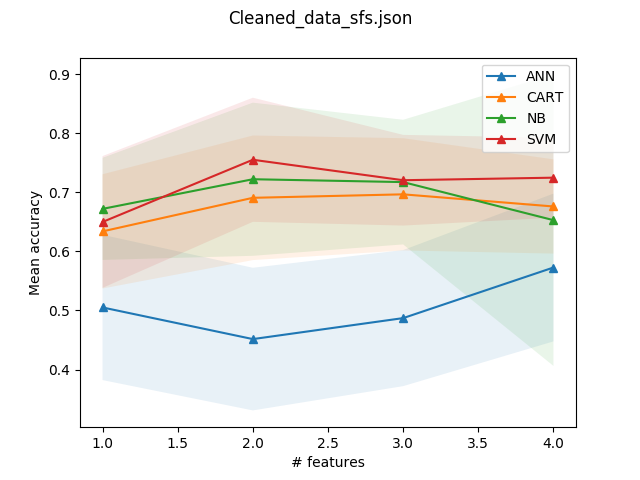
\includegraphics[width=\textwidth]{../plots_with_std_fill/Cleaned_data_sf_combined.png}
      \caption[]%
      {{\small Dataset EN using SFS}}
      \label{fig:EN_sfs}
  \end{subfigure}
  \hfill
  \begin{subfigure}[b]{0.475\textwidth}
      \centering
      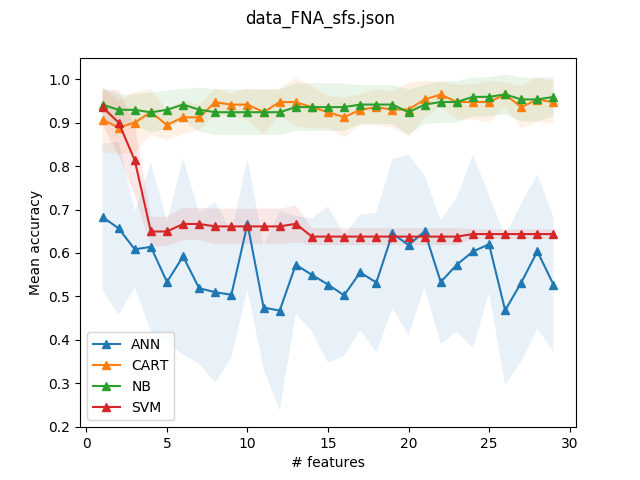
\includegraphics[width=\textwidth]{../plots_with_std_fill/data_FNA_sf_combined.png}
      \caption[]%
      {{\small Dataset WBCD using SFS}}
      \label{fig:WBCD_sfs}
  \end{subfigure}
  \vskip\baselineskip
  \begin{subfigure}[b]{0.475\textwidth}
      \centering
      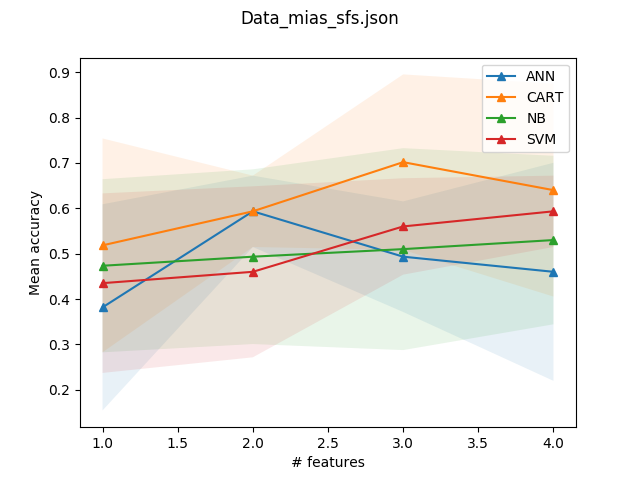
\includegraphics[width=\textwidth]{../plots_with_std_fill/Data_mias_sf_combined.png}
      \caption[]%
      {{\small Dataset MIAS using SFS}}
      \label{fig:MIAS_sfs}
  \end{subfigure}
  \quad
  \begin{subfigure}[b]{0.475\textwidth}
      \centering
      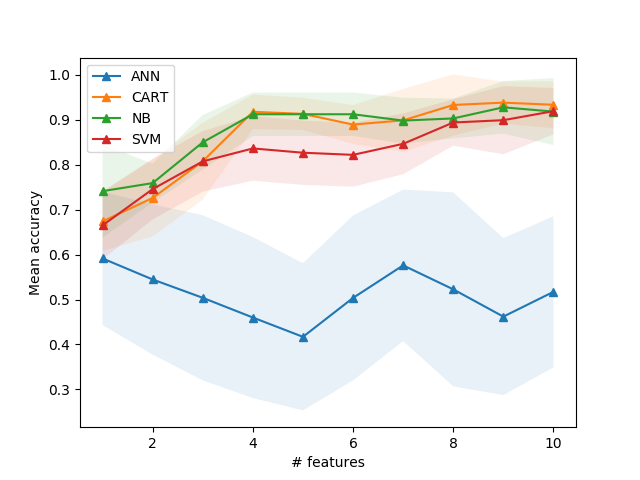
\includegraphics[width=\textwidth]{../plots_with_std_fill/FNA_gb_sf_combined.png}
      \caption[]%
      {{\small Dataset RHH using SFS}}
      \label{fig:RHH_sfs}
  \end{subfigure}
  \caption[]
  {{\small Combined plots of all datasets comparing each classifier when using SFS for feature selection.}}
  \label{fig:plots_sfs}
\end{figure*}
